% Informe IEEE - Proyecto Integrador IA Avanzada - Ruta A - Reto A1
% Compilar en Overleaf (pdfLaTeX + BibTeX). Si el curso entrega su propia plantilla,
% copiar el contenido de cada sección en ella. Extensión exigida: 6 a 8 páginas.
\documentclass[conference]{IEEEtran}
\usepackage[spanish,es-tabla]{babel}
\usepackage[utf8]{inputenc}
\usepackage[T1]{fontenc}  % tildes correctas al copiar y buscar texto en el PDF
\usepackage{cite}
\usepackage{amsmath}
\usepackage{graphicx}
\usepackage{booktabs}
\usepackage{url}
\graphicspath{{../../reports/figures/}{./}{figures/}}  % en Overleaf basta subir las imágenes junto al .tex

\begin{document}

\title{La voz del usuario: clasificación de sentimiento y extracción de quejas en reseñas de aplicaciones bancarias colombianas, y por qué las estrellas engañan}

\author{\IEEEauthorblockN{Elias Jaramillo}
\IEEEauthorblockA{Inteligencia Artificial Avanzada -- Proyecto Integrador (Ruta A)\\
Fundación Universitaria Compensar -- Bogotá, Colombia\\
edjaramillo@ucompensar.edu.co}}

\maketitle

\begin{abstract}
% 150-250 palabras: problema, datos, método, resultado principal (con número), conclusión.
Las aplicaciones bancarias más usadas en Colombia reciben miles de reseñas al mes que nadie analiza de forma
sistemática. Este trabajo construye un corpus anonimizado de 11.569 reseñas en español de Nequi, Daviplata y
Bancolombia. Para clasificar el sentimiento en tres clases compara una línea base TF-IDF con regresión logística,
una red BiLSTM, el modelo BETO con ajuste fino y el modelo preentrenado pysentimiento sin ajuste. Los modelos
ajustados se entrenan con una etiqueta débil derivada de las estrellas y todos se evalúan sobre 300 reseñas con
etiqueta revisada por humano. BETO supera a la línea base (F1-macro 0,651 frente a 0,606), pero el mejor resultado
lo obtiene pysentimiento sin ajuste (0,740), con un recall de 0,946 en la clase negativa. El análisis muestra que
las estrellas son una etiqueta ruidosa: solo 2 de 12 reseñas de tres estrellas son realmente neutras. Ese ruido
limita a los modelos ajustados y, si se evaluara con estrellas, llevaría a escoger el modelo equivocado.
Las palabras clave (YAKE) y los temas de queja muestran que el problema dominante es no poder ingresar a la app:
lo menciona el 56\,\% de las quejas de Daviplata, ligado a un ciclo de actualización fallida. En Bancolombia
predominan las caídas y la lentitud.
\end{abstract}

\begin{IEEEkeywords}
análisis de sentimiento, procesamiento de lenguaje natural, BETO, BiLSTM, reseñas de aplicaciones, banca digital
\end{IEEEkeywords}

\section{Introducción}
En Colombia, buena parte de la relación entre los usuarios y su banco pasa por el celular. Aplicaciones como Nequi,
Daviplata y Bancolombia se usan para pagar, transferir y retirar dinero, y cuando fallan el usuario no puede usar su
plata. La tienda Google Play se convierte entonces en un canal de quejas público. Solo en la descarga hecha para este
trabajo, Daviplata acumuló 4.411 reseñas distintas en cinco meses (unas 880 al mes) y Nequi 3.279 en dos meses.

Ese volumen supera lo que un equipo puede leer. El \textbf{dueño del problema} es el área de experiencia de cliente
o de producto digital de cada banco. Necesita saber dos cosas: de qué se quejan los usuarios y si la situación mejora
después de cada versión de la app. Hoy esa lectura no se hace de forma sistemática, y las estrellas no bastan: como
se muestra en este trabajo, muchas reseñas con cuatro o cinco estrellas son quejas.

El análisis de sentimiento resuelve este tipo de problema \cite{liu2012sentiment}, y existen modelos preentrenados
para español \cite{canete2020beto,perez2021pysentimiento}. Sin embargo, entrenarlos con datos propios exige
etiquetas, y la fuente gratuita de etiquetas, las estrellas, es ruidosa. Este trabajo mide cuánto afecta ese ruido.

El objetivo es construir y evaluar un sistema que clasifique el sentimiento de las reseñas en tres clases y resuma
las quejas más frecuentes por app y por mes. Las contribuciones de este trabajo son: (i) un corpus anonimizado de 11.569 reseñas, con 300 de evaluación revisadas
por humano; (ii) una comparación entre una línea base clásica, dos redes profundas entrenadas por el autor y un modelo
preentrenado; (iii) evidencia de que la etiqueta por estrellas limita el ajuste fino y engaña si se usa para evaluar;
(iv) un análisis de quejas por app y por mes; y (v) una demo reproducible.

\section{Trabajos relacionados}
\textbf{Enfoques clásicos.} El análisis de sentimiento clasifica la opinión expresada en un texto
\cite{liu2012sentiment}. La forma clásica representa cada texto como una bolsa de palabras ponderada con TF-IDF y
entrena un clasificador lineal, como la regresión logística \cite{pedregosa2011sklearn}. Es rápida, interpretable
y difícil de superar con pocos datos, por eso se usa aquí como línea base. Su límite es que ignora el orden de las
palabras: no distingue bien ``no es buena'' de ``es buena, no falla''.

\textbf{Redes recurrentes.} Las redes LSTM \cite{hochreiter1997lstm} leen el texto en secuencia y conservan memoria
de lo leído. La versión bidireccional (BiLSTM) \cite{schuster1997bidirectional} lo lee en ambos sentidos, de modo que
cada palabra se interpreta con su contexto a la izquierda y a la derecha.

\textbf{Transformers preentrenados.} El Transformer \cite{vaswani2017attention} reemplaza la recurrencia por
mecanismos de atención. BERT \cite{devlin2019bert} lo preentrena con grandes cantidades de texto, y después basta un
ajuste fino corto para una tarea concreta. BETO \cite{canete2020beto} es la versión de BERT entrenada con texto en
español. La librería Transformers \cite{wolf2020transformers} facilita el ajuste fino de estos modelos.

\textbf{Sentimiento en español.} pysentimiento \cite{perez2021pysentimiento} ofrece modelos listos para usar en
español, basados en RoBERTuito \cite{perez2022robertuito}, un modelo preentrenado con texto de redes sociales y
ajustado con corpus de sentimiento anotados a mano. Por eso sirve como referencia: no depende de las estrellas.

\textbf{Palabras clave y explicabilidad.} YAKE \cite{campos2020yake} extrae palabras clave de un texto sin
entrenamiento, con estadísticas locales (frecuencia, posición y dispersión de cada término). Para explicar las
predicciones se usan los coeficientes de la regresión logística y SHAP \cite{lundberg2017shap}, que reparte la
predicción entre las palabras de entrada según los valores de Shapley.

\section{Datos}
\subsection{Fuente y recolección}
Se descargaron las 5.000 reseñas más recientes de cada app en Google Play con la librería
\texttt{google-play-scraper} (idioma español, país Colombia) el 16 de noviembre de 2026. La fecha queda registrada
en \texttt{data/raw/metadatos\_descarga.json}. Las reseñas son públicas y se usan solo con fines académicos.
Al quitar textos vacíos y duplicados quedan 11.569 reseñas (Tabla~\ref{tab:datos}).
\subsection{Anonimización y ética}
Se eliminan nombres e imágenes, el identificador se reemplaza por un hash y se enmascaran correos y números
largos, de acuerdo con la Ley 1581 de 2012 \cite{ley1581}.
\subsection{Análisis exploratorio}
El corpus tiene 11.569 reseñas, cada una con texto, estrellas (1 a 5), fecha, app, número de ``me gusta'' y
versión de la app. Después de la limpieza el texto y las estrellas no tienen faltantes; las demás columnas no se
usan en los modelos.

\textbf{Desbalance.} Por estrellas, el 56,3\,\% de las reseñas es negativa (1--2), solo el 5,7\,\% neutra (3) y el
38,1\,\% positiva (4--5). Las estrellas se concentran en los extremos: 5.729 reseñas tienen una estrella y 3.762 tienen
cinco. Por eso se usan pesos de clase al entrenar y F1-macro para evaluar. El desbalance cambia mucho entre apps
(Tabla~\ref{tab:datos}): Daviplata tiene 72,5\,\% de reseñas negativas y Nequi solo 28,5\,\%.

\textbf{Longitud.} Las reseñas son cortas: mediana de 12 palabras, media de 18,2 y percentil 90 de 43 palabras
(máximo 111). El 17,7\,\% tiene tres palabras o menos (``excelente'', ``no entra''). Por eso se fijó una longitud
máxima de 80 tokens para la BiLSTM y de 128 para BETO: cubre casi todas las reseñas sin cortarlas
(Fig.~\ref{fig:eda}).
\subsection{Etiquetado}
Etiqueta débil por estrellas (1--2 negativa, 3 neutra, 4--5 positiva) para entrenar. Para evaluar se usan 300
reseñas separadas desde el inicio. Un modelo de lenguaje (Claude, Anthropic) las pre-etiquetó leyendo solo el texto,
sin las estrellas y con las reglas de la guía de etiquetado. Luego el autor revisó a mano todas las reseñas en las que
esa etiqueta no coincidía con las estrellas (42 casos) y una muestra aleatoria de 30 en las que sí coincidía.
En la revisión se corrigieron 2 de las 72 etiquetas revisadas (2,8\,\%). El modelo de lenguaje que etiquetó no es
ninguno de los modelos evaluados, así que no hay evaluación circular.

La etiqueta final queda con 184 negativas, 15 neutras y 101 positivas, y coincide con las estrellas en el 86,7\,\%
de los casos. La Tabla~\ref{tab:estrellas} muestra dónde fallan las estrellas: 17 reseñas con 4--5 estrellas son en
realidad quejas, y de las 12 reseñas con 3 estrellas solo 2 son neutras (8 son negativas).

\begin{table}[t]
\caption{Etiqueta débil (estrellas) frente a etiqueta revisada en las 300 reseñas de evaluación}
\label{tab:estrellas}
\centering
\begin{tabular}{lrrrr}
\toprule
Estrellas $\backslash$ Revisada & Negativa & Neutra & Positiva & Total \\
\midrule
Negativa (1--2) & 159 & 2 & 0 & 161 \\
Neutra (3) & 8 & 2 & 2 & 12 \\
Positiva (4--5) & 17 & 11 & 99 & 127 \\
\midrule
Total & 184 & 15 & 101 & 300 \\
\bottomrule
\end{tabular}
\end{table}

\begin{table}[t]
\caption{Reseñas por aplicación}
\label{tab:datos}
\centering
\begin{tabular}{lrrr}
\toprule
App & Reseñas & \% neg. (estrellas) & Periodo principal \\
\midrule
Nequi & 3.279 & 28,5 & sep.--nov. 2026 \\
Daviplata & 4.411 & 72,5 & jul.--nov. 2026 \\
Bancolombia & 3.879 & 61,2 & jun. 2024--may. 2025 \\
\midrule
Total & 11.569 & 56,3 & \\
\bottomrule
\end{tabular}
\end{table}

\begin{figure}[t]
\centering
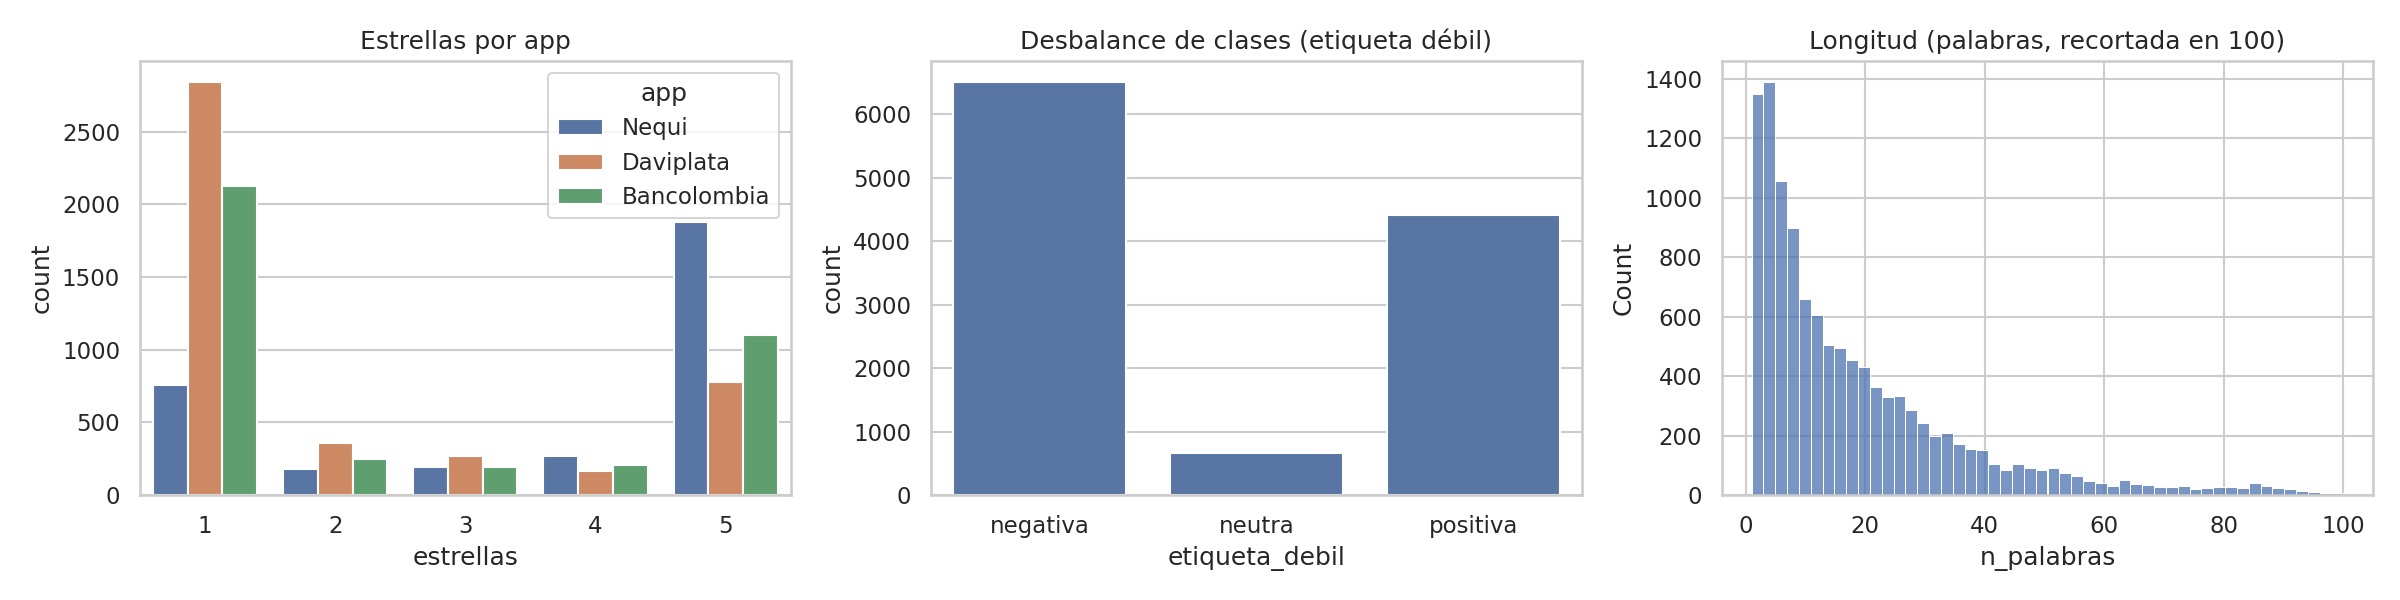
\includegraphics[width=\columnwidth]{eda_distribuciones.png}
\caption{Distribución de estrellas, desbalance de clases y longitud de las reseñas.}
\label{fig:eda}
\end{figure}

\section{Metodología}
\subsection{División de los datos}
Primero se separan las 300 reseñas de evaluación (100 por app, al azar). El resto se divide en entrenamiento
(9.015), validación (1.127) y prueba (1.127), estratificado por la etiqueta débil y con semilla 42. Todo esto ocurre
\emph{antes} de construir cualquier vocabulario, TF-IDF o tokenizador, para que no haya fuga de información. La
validación se usa para elegir hiperparámetros; las 300 de evaluación solo se usan al final.

\subsection{Línea base}
TF-IDF de unigramas y bigramas (hasta 50.000 términos, frecuencia mínima 2) con regresión logística
\cite{pedregosa2011sklearn} y pesos de clase balanceados. El parámetro de regularización $C$ se eligió entre
$\{0{,}1;\,0{,}3;\,1;\,3;\,10\}$ por el F1-macro en validación.

\subsection{BiLSTM}
Vocabulario de 20.000 palabras construido solo con entrenamiento, secuencias de 80 tokens, \emph{embedding} de 128
dimensiones entrenado desde cero, una capa BiLSTM de 64 unidades por dirección
\cite{hochreiter1997lstm,schuster1997bidirectional}, \emph{dropout} de 0,4 y salida \emph{softmax}. Se entrenó con Adam
($10^{-3}$), lote de 64 y pesos de clase. Con \emph{early stopping} (paciencia 2) el entrenamiento se detuvo en la
cuarta época y conservó los pesos de la segunda, donde la pérdida de validación fue mínima (0,61); después la
pérdida de entrenamiento siguió bajando mientras la de validación subía, señal de sobreajuste.

\subsection{BETO con ajuste fino}
Modelo \texttt{bert-base-spanish-wwm-cased} \cite{canete2020beto} con la librería Transformers
\cite{wolf2020transformers}. Hiperparámetros: tasa de aprendizaje $2\times10^{-5}$, 3 épocas, lote de 32, longitud
máxima de 128 tokens, 10\,\% de pasos de calentamiento y decaimiento de pesos de 0,01. Son los valores recomendados
para ajustar BERT \cite{devlin2019bert}: una tasa baja y pocas épocas evitan borrar lo que el modelo aprendió en el
preentrenamiento. La pérdida de entropía cruzada se ponderó por clase, y se guardó la época con mejor F1-macro en
validación. Se entrenó en una GPU T4 de Google Colab.

\subsection{Referencia sin ajuste}
El analizador de sentimiento de pysentimiento \cite{perez2021pysentimiento}, basado en RoBERTuito
\cite{perez2022robertuito}, se aplicó tal cual, sin entrenarlo con nuestros datos. Responde una pregunta práctica:
¿vale la pena ajustar un modelo propio frente a uno listo para usar?

\subsection{Componente NLP de quejas}
Con el mejor modelo se clasifica todo el corpus. Sobre las reseñas negativas se calculan: (i) el porcentaje de
reseñas negativas por app y por mes (solo meses con al menos 30 reseñas); (ii) palabras clave con YAKE
\cite{campos2020yake}, quitando términos genéricos del dominio (``app'', el nombre del banco); y (iii) temas de queja
detectados con reglas de palabras (acceso, actualización, compatibilidad, caídas, clave, pagos, atención y cobros).

\subsection{Métrica}
La métrica principal es el F1-macro sobre las 300 reseñas de evaluación:
\begin{equation}
F1_{macro} = \frac{1}{K}\sum_{k=1}^{K} \frac{2\,P_k R_k}{P_k + R_k}
\end{equation}
donde $K=3$ y $P_k$, $R_k$ son la precisión y el recall de la clase $k$. Se eligió porque las clases están
desbalanceadas: la exactitud premiaría a un modelo que dijera siempre ``negativa'' (acertaría el 61\,\%). El F1-macro,
en cambio, le da el mismo peso a cada clase. Como métrica secundaria se usa el recall de la clase negativa, porque
una queja no detectada es el error más costoso para el dueño del problema.

\section{Resultados}
\begin{table}[t]
\caption{Resultados en el conjunto de oro (300 reseñas, etiqueta revisada) y en el test con etiqueta débil (1.127 reseñas)}
\label{tab:resultados}
\centering
\setlength{\tabcolsep}{4pt}
\begin{tabular}{lcccc}
\toprule
 & \multicolumn{3}{c}{Oro (principal)} & Test débil \\
Modelo & F1-macro & Rec. neg. & Exactitud & F1-macro \\
\midrule
TF-IDF + RegLog (base) & 0,606 & 0,815 & 0,833 & 0,620 \\
BiLSTM & 0,613 & 0,783 & 0,810 & 0,609 \\
BETO ajuste fino & 0,651 & 0,799 & 0,833 & \textbf{0,628} \\
pysentimiento (sin ajuste) & \textbf{0,740} & \textbf{0,946} & \textbf{0,870} & 0,535 \\
\bottomrule
\end{tabular}
\end{table}

\begin{figure*}[t]
\centering
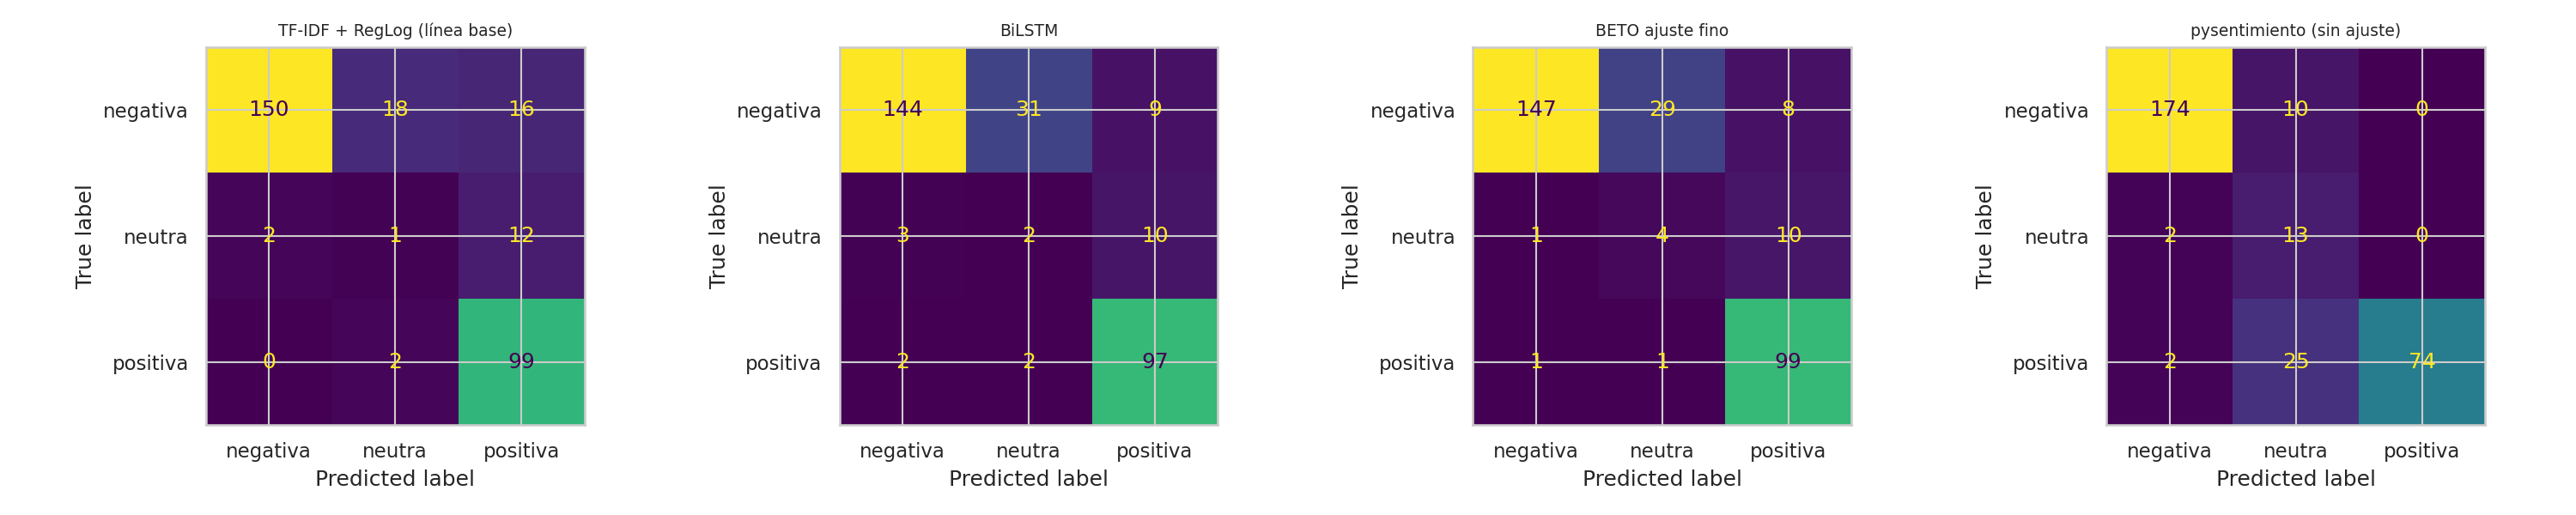
\includegraphics[width=\textwidth]{matrices_confusion_oro.png}
\caption{Matrices de confusión en las 300 reseñas de evaluación (filas: etiqueta revisada; columnas: predicción).}
\label{fig:confusion}
\end{figure*}

La Tabla~\ref{tab:resultados} resume los resultados. Las dos redes profundas entrenadas por el autor superan a la
línea base en F1-macro: la BiLSTM por poco (+0,007) y BETO por 4,5 puntos (0,651 frente a 0,606). Sin embargo, el
mejor modelo es pysentimiento sin ajuste, con F1-macro de 0,740 y recall de 0,946 en la clase negativa: detecta
174 de las 184 quejas, frente a 147 de BETO y 150 de la línea base.

Las matrices de confusión (Fig.~\ref{fig:confusion}) muestran de dónde viene la diferencia. Los tres modelos
entrenados con estrellas casi nunca aciertan la clase neutra (1 a 4 de 15) y confunden muchas quejas con neutras
(BETO: 29; BiLSTM: 31). En las estrellas, la clase ``neutra'' (3 estrellas) es sobre todo quejas moderadas, y eso es lo que
aprendieron. pysentimiento, entrenado con otro corpus anotado a mano, no hereda ese ruido. Su punto débil es el
opuesto: etiqueta como neutras 25 reseñas positivas cortas (``Bie'', ``exc'', ``cool''), así que la precisión de la
clase neutra es de solo 0,271 (F1 neutra 0,413, frente a 0,961 en la negativa y 0,846 en la positiva).

El resultado más importante para la metodología está en la última columna: \textbf{si se evaluara con las estrellas,
el ranking se invertiría}. pysentimiento quedaría último (0,535) y BETO primero (0,628). Evaluar con la etiqueta
débil habría llevado a escoger el peor modelo para el dueño del problema.

Como la clase neutra tiene solo 15 ejemplos, cada acierto en ella mueve el F1-macro varios puntos. Por eso también
se reporta el recall de la clase negativa, que es la que más le importa al dueño: una queja no detectada es una
queja que nadie atiende.

\subsection{Quejas por app y por mes}
Con el mejor modelo se clasificó todo el corpus: 3.706 reseñas negativas de Daviplata, 2.557 de Bancolombia y
1.218 de Nequi. La Tabla~\ref{tab:temas} muestra qué porcentaje de esas reseñas menciona cada tema de queja, y la
Tabla~\ref{tab:kw} las palabras clave que extrajo YAKE después de quitar términos genéricos.

\begin{table}[t]
\caption{Porcentaje de reseñas negativas que mencionan cada tema}
\label{tab:temas}
\centering
\begin{tabular}{lrrr}
\toprule
Tema & Bancolombia & Daviplata & Nequi \\
\midrule
Acceso / no deja entrar & 19,8 & \textbf{56,2} & \textbf{39,9} \\
Actualización & 14,3 & 35,1 & 5,3 \\
Compatibilidad del celular & 9,8 & 3,9 & 1,0 \\
Caídas / lentitud & \textbf{25,1} & 13,4 & 21,8 \\
Clave / verificación & 9,9 & 3,0 & 9,4 \\
Transferencias / pagos & 24,6 & 36,4 & 23,0 \\
Atención al cliente & 4,2 & 8,3 & 4,8 \\
Cobros / comisiones & 2,6 & 0,3 & 1,8 \\
\bottomrule
\end{tabular}
\end{table}

\begin{table}[t]
\caption{Palabras clave (YAKE) de las reseñas negativas por app}
\label{tab:kw}
\centering
\begin{tabular}{p{0.2\columnwidth}p{0.7\columnwidth}}
\toprule
App & Palabras clave \\
\midrule
Bancolombia & clave dinámica, celular, compatible, mantiene caída, caída, lenta, ingresar, dinero \\
Daviplata & ingresar, dinero, pide actualizar, abrir, entrar, actualizar, instalar, intentando ingresar \\
Nequi & entrar, dinero, abrir, reconocimiento facial, ingresar, tarjeta, problema \\
\bottomrule
\end{tabular}
\end{table}

\begin{figure}[t]
\centering
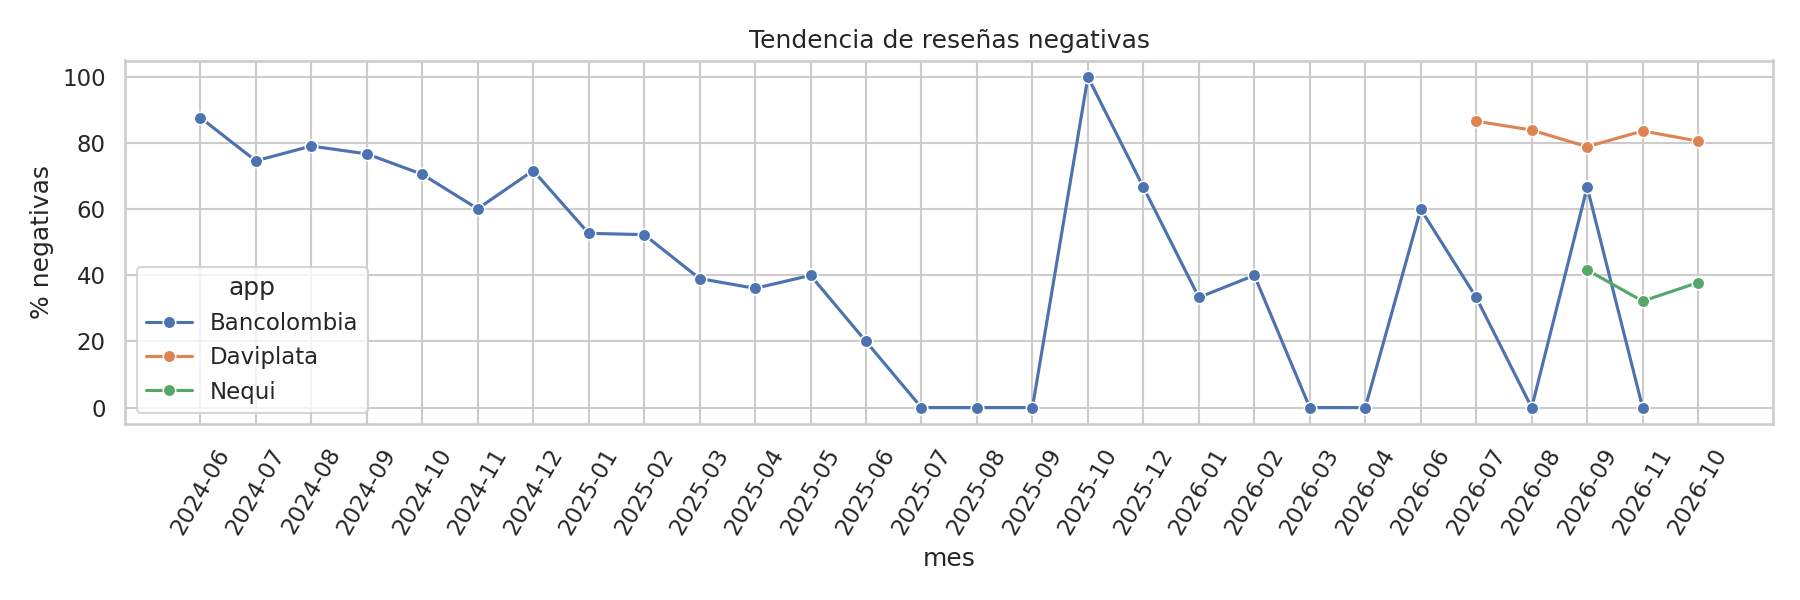
\includegraphics[width=\columnwidth]{tendencia_negativas.png}
\caption{Porcentaje de reseñas negativas por mes (solo meses con al menos 30 reseñas).}
\label{fig:tendencia}
\end{figure}

Cada app tiene un problema dominante distinto:
\begin{itemize}
\item \textbf{Daviplata} vive una crisis de acceso: el 56\,\% de sus quejas dice que no puede entrar y el 35\,\% menciona
una actualización. Las palabras clave (\emph{pide actualizar}, \emph{instalar}, \emph{intentando ingresar}) describen un
ciclo: la app pide actualizar, la tienda no ofrece la actualización y reinstalar no lo resuelve. Entre julio y noviembre
de 2026, entre el 79\,\% y el 87\,\% de sus reseñas son negativas (Fig.~\ref{fig:tendencia}).
\item \textbf{Bancolombia} concentra sus quejas en caídas y lentitud (25\,\%) y en la compatibilidad con celulares
antiguos (9,8\,\%, el valor más alto de las tres). Entre junio de 2024 y mayo de 2025 el porcentaje de reseñas
negativas bajó de 88\,\% a cerca de 40\,\%.
\item \textbf{Nequi} tiene la menor proporción de reseñas negativas (32\,\% a 42\,\%, con tendencia a la baja).
Sus quejas se reparten entre acceso (40\,\%) y validación de identidad (\emph{reconocimiento facial}).
\end{itemize}

\textbf{Advertencia sobre los periodos.} Como se descargaron las 5.000 reseñas más recientes de cada app, los
periodos no coinciden. Casi todas las reseñas de Bancolombia son de junio de 2024 a mayo de 2025; después solo
aparecen reseñas esporádicas, menos de 30 al mes. Eso sugiere que el identificador descargado corresponde a la
versión anterior de la app (varias reseñas hablan de la ``nueva app''). Daviplata va de julio a noviembre de 2026,
y Nequi de septiembre a noviembre de 2026. Por eso las tendencias sirven para cada app por
separado, pero no para comparar apps en el mismo mes.
\subsection{Análisis de errores}
El mejor modelo se equivoca en 39 de las 300 reseñas. Se revisaron y comentaron las 39 (archivo
\texttt{reports/analisis\_errores.csv}) y se agruparon por causa (Tabla~\ref{tab:errores}). El patrón es claro: en
35 de los 39 errores el modelo predice \emph{neutra}, sobre todo en textos muy cortos o mal escritos.

\begin{table}[t]
\caption{Causas de los 39 errores de pysentimiento en el conjunto de oro}
\label{tab:errores}
\centering
\begin{tabular}{p{0.62\columnwidth}r}
\toprule
Causa & Errores \\
\midrule
Ortografía, abreviatura o jerga (``exelecte'', ``exc'', ``super full'', ``nomedeja'') & 17 \\
Elogio funcional sin palabras de emoción (``me facilita y agiliza pagos'') & 6 \\
Queja descrita como hecho técnico (``no me crea la clave dinámica'') & 6 \\
Texto muy corto con sesgo hacia neutra (``No entra'', ``Es bueno'') & 6 \\
Reseña mixta o etiqueta discutible & 4 \\
\midrule
Total & 39 \\
\bottomrule
\end{tabular}
\end{table}

Los errores no cuestan lo mismo. Los 25 casos de positiva clasificada como neutra son baratos: solo subestiman la
satisfacción. Los 10 casos de \textbf{queja no detectada} son los costosos, porque nadie atendería esa queja. Siete
de esos 10 son fallas técnicas contadas sin palabras negativas (``No permite el ingreso a la plataforma aún cuando tengo
el usuario y contraseña intactos'') o con la negación pegada (``nomedeja''). El modelo se entrenó con tuits, que expresan
la emoción de forma explícita; en una tienda de apps, en cambio, muchos usuarios solo describen la falla. Esto
sugiere ajustar el modelo con reseñas de tiendas de aplicaciones.
\subsection{Explicabilidad}
\begin{figure*}[t]
\centering
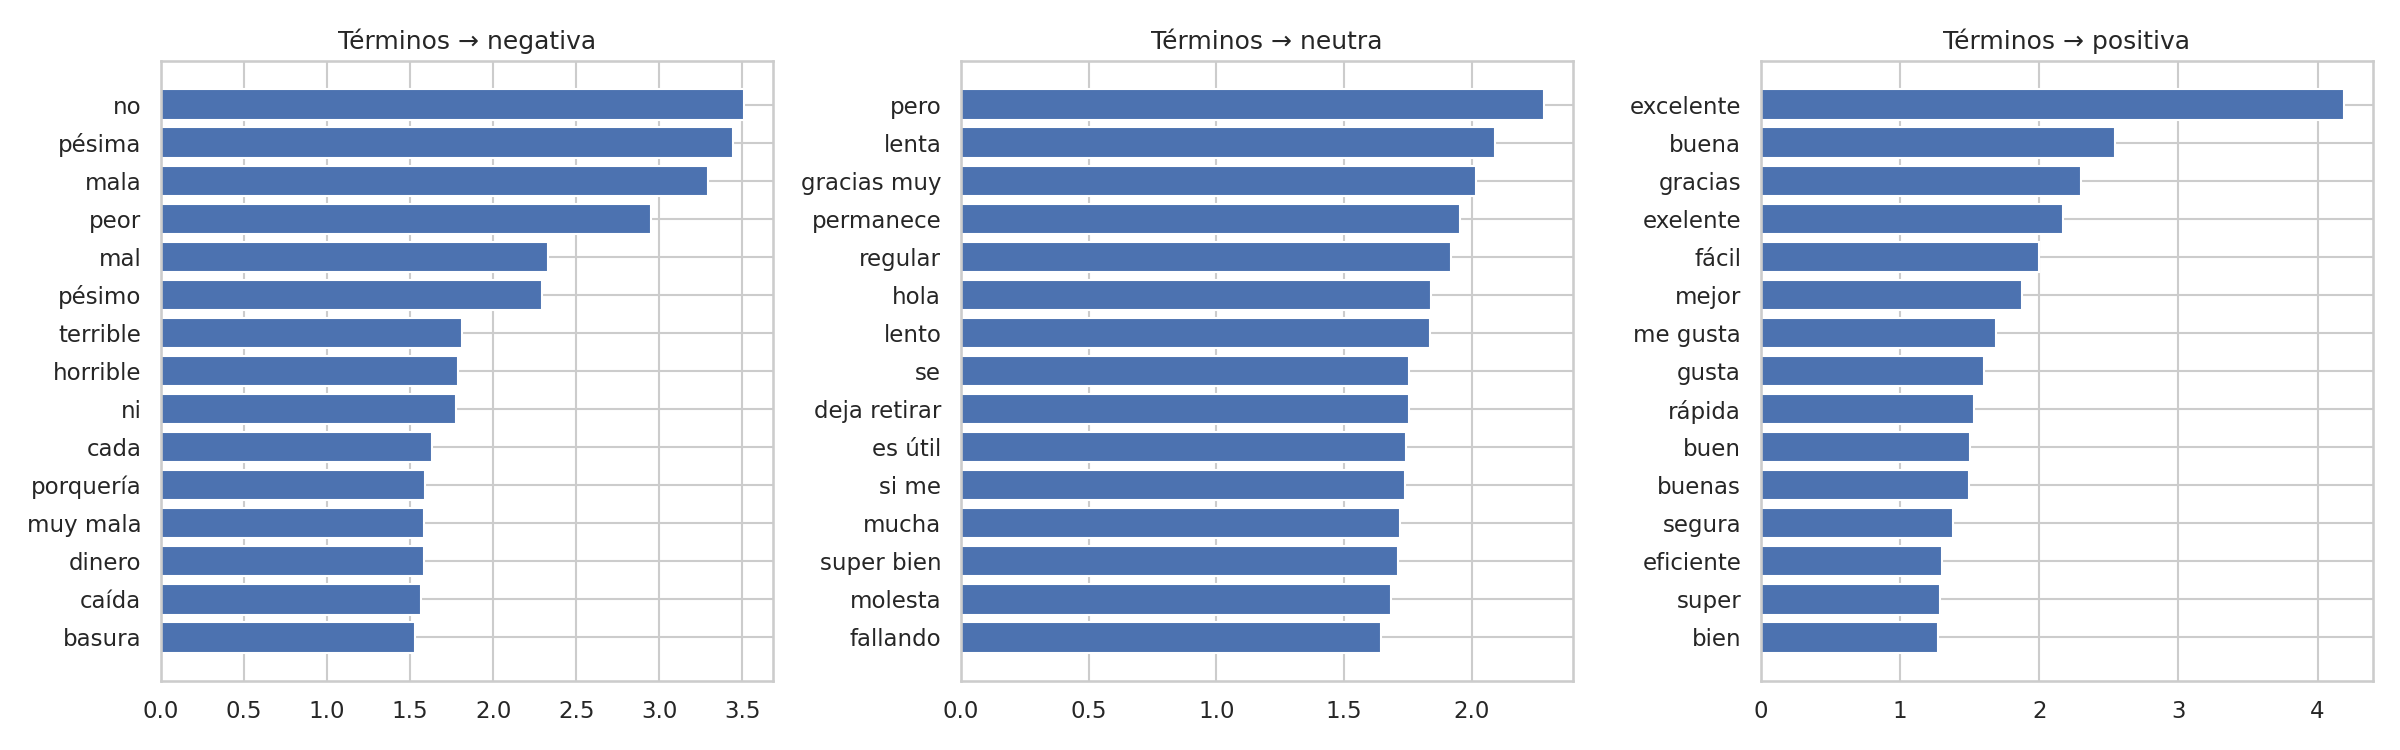
\includegraphics[width=\textwidth]{explicabilidad_coeficientes.png}
\caption{Los 15 términos con mayor coeficiente por clase en la línea base (TF-IDF + regresión logística).}
\label{fig:coef}
\end{figure*}

La Fig.~\ref{fig:coef} muestra los términos que más empujan cada decisión de la línea base. Para \emph{negativa} y
\emph{positiva} los términos tienen sentido: ``no'', ``pésima'', ``mala'', ``peor'', ``caída'' y ``basura'' frente a
``excelente'', ``buena'', ``fácil'', ``me gusta'' y ``segura''. El modelo aprendió incluso variantes mal escritas como
``exelente''.

La clase \emph{neutra} explica el problema central de este trabajo. Sus términos más fuertes son ``pero'',
``lenta'', ``lento'', ``fallando'', ``molesta'' y ``deja retirar''. No son palabras neutrales: son \textbf{quejas
moderadas}. El modelo aprendió de las estrellas que ``3 estrellas'' significa ``queja suave'', y por eso confunde
quejas con neutras en la evaluación. La explicabilidad confirma con otra evidencia lo que mostraron la
Tabla~\ref{tab:estrellas} y las matrices de confusión.
% Si la celda de SHAP corrió en el notebook, agregar aquí una captura con 2 ejemplos y comentarla \cite{lundberg2017shap}.

\section{Discusión}
\textbf{Qué funcionó.} El ajuste fino de BETO mejora a la línea base y a la BiLSTM, lo que confirma la ventaja
de un Transformer preentrenado en español sobre la bolsa de palabras y sobre embeddings aprendidos desde cero con
9.015 ejemplos. El modelo preentrenado para sentimiento fue aún mejor sin necesidad de entrenamiento.

\textbf{Qué no funcionó.} El ajuste fino no superó a pysentimiento. La causa principal es la etiqueta débil: 13,3\,\%
de las estrellas no coinciden con el texto, y la clase de 3 estrellas casi nunca es neutra. Un modelo con más capacidad
aprende mejor ese ruido, no menos. Los modelos entrenados con estrellas también salen mejor evaluados con estrellas, lo que
muestra que medir con la misma fuente ruidosa con la que se entrena sobreestima el desempeño.

\textbf{Límites.} (i) El conjunto de evaluación tiene solo 15 neutras. (ii) Lo pre-etiquetó un modelo de lenguaje y
solo se revisaron a mano los casos dudosos y una muestra de control. (iii) En Google Play escriben más los usuarios
muy molestos o muy satisfechos. (iv) Los periodos no coinciden entre apps: Bancolombia se concentra en 2024--2025,
probablemente por corresponder a la versión anterior de su app, y las otras dos en 2026. (v) Los temas de queja se detectan con reglas de palabras,
que no reconocen sinónimos ni errores de ortografía.

\section{Conclusiones}
Para clasificar reseñas bancarias en español, un modelo preentrenado de sentimiento (pysentimiento) detecta el
94,6\,\% de las quejas y supera a los modelos ajustados con estrellas (F1-macro 0,740 frente a 0,651 de BETO y
0,606 de la línea base). Las estrellas son una etiqueta barata, pero ruidosa: limitan el ajuste fino y no sirven
para evaluar, porque con ellas se habría elegido el peor modelo. El análisis de quejas muestra que el problema
dominante es el acceso a la app, con una crisis clara en Daviplata ligada a una actualización que no se puede instalar.

\textbf{¿Qué tan lejos está de que el dueño lo use?} El clasificador y el tablero ya funcionan y responden las dos
preguntas del dueño: de qué se quejan los usuarios y cómo cambia eso mes a mes. Para usarlo de verdad faltan tres
cosas: descargar las reseñas de forma automática cada semana, incluir la app nueva de Bancolombia y App Store, y
reemplazar las reglas de temas por un modelo que reconozca sinónimos y errores de ortografía.

\textbf{¿En qué se equivoca y qué cuesta cada error?} Se equivoca sobre todo con textos muy cortos, mal escritos o
que describen una falla sin palabras negativas. Clasificar un elogio como neutro es barato: solo subestima la
satisfacción. No detectar una queja es caro: un problema real (por ejemplo, ``no me crea la clave dinámica'') queda
fuera del conteo y puede retrasar su solución. Por eso se prioriza el recall de la clase negativa.

\textbf{¿A quién podría perjudicar?} Las reseñas escritas con mala ortografía o jerga tienen más probabilidad de
clasificarse mal, así que la voz de los usuarios con menos escolaridad o de ciertas regiones podría quedar
subrepresentada. Tampoco se debe usar el sistema para juzgar a usuarios individuales ni para decidir
respuestas automáticas sin revisión humana. Además, un porcentaje alto de quejas describe la experiencia de quienes
escriben reseñas, no la de todos los clientes.

\textbf{¿Qué haría con un mes más y el doble de datos?} (i) Etiquetar a mano unas 1.000 reseñas, con más neutras,
y ajustar pysentimiento o BETO con ellas en vez de con estrellas. (ii) Descargar las tres apps en el mismo periodo.
(iii) Reemplazar las reglas de temas por modelado de temas (BERTopic). (iv) Normalizar la ortografía antes de
clasificar (``exelente'' → ``excelente'', ``nomedeja'' → ``no me deja'').

\section*{Declaración de uso de IA generativa}
Se usó Claude (Anthropic) como asistente para estructurar el código del notebook y la demo, apoyar la redacción
de este informe y proponer la clasificación de los errores, y para pre-etiquetar las 300 reseñas de evaluación, que el
autor revisó según el procedimiento de la Sección~III.
Todo el código fue ejecutado, revisado y comprendido por el autor; los resultados y su interpretación son propios.

\section*{Disponibilidad}
Código y datos procesados: \url{https://github.com/A-P-O-L-O/la-voz-del-usuario}.

\bibliographystyle{IEEEtran}
\bibliography{referencias}

\end{document}
